\item Determine la carga vertical por unidad de área, ejercida sobre el vehículo, debida al efecto suelo (producida por el flujo de aire alrededor del mismo). Para ello considere el volumen de control graficado en líneas de trazo y punto, y suponga un ancho del vehículo constante. Además suponga que la presión en la superficie libre superior del vehículo, coincide con la presión a la entrada del volumen de control. Considere los perfiles de velocidades como uniformes.

$$A_{ent} = A_{sal} \qquad A_{sup} = c_{sup}\,A_{ent} \qquad A_{inf} = c_{inf}\,A_{ent} $$

$$c_{sup} = 0,5 \qquad c_{inf} = 0,25$$

$$V_{ent} = 80 \text{km/h} \qquad V_{sup}=85 \text{km/h} \qquad P_{ent} = P_{sal} = P_{atm} = 100000\text{Pa}$$
%% Esto es una figura

\begin{figure}[h]
\centering
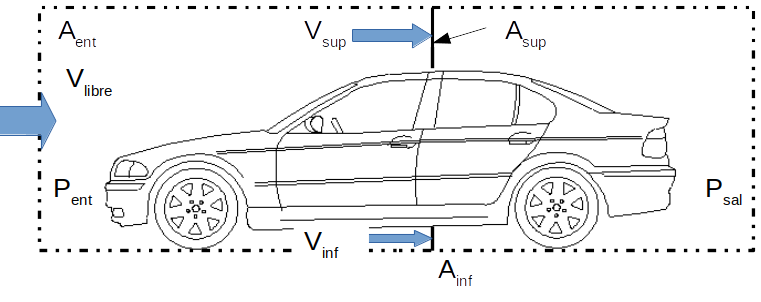
\includegraphics[width=0.7\textwidth]{vehiculo.png}
\caption{flujo alrededor de vehículo}
\label{fig:vehiculo}
\end{figure}

